\section{跨文件编译}
我们曾谈过,一个源代码的核心是主函数 \lstinline@main@。为了突出重点,我们更倾向于把主函数的定义放在其它函数的定义之前。这样就会带来``找不到函数''的问题,因为编译器在遇到一个函数名的时候,它会先向前寻找。\par
为了解决这个问题,我们需要在函数的定义之前先声明。如果有默认值的话,也尽量放在函数声明的时候写出来,否则编译器也找不到它。\par
我们后来又学习了结构体、共用体和类。它们也遵循这样的规则,我们必须在使用它之前就给出声明。
\begin{lstlisting}
class Data; //Data类的声明
void func(Data); //func(Data)的声明
//...
class Data {
    //...
}; //Data的定义
void func(Data d) {
    //...
} //func(Data)的定义
\end{lstlisting}
其中 \lstinline@Data@ 的声明和 \lstinline@func(Data)@ 的声明是不能颠倒的,否则编译器就找不到 \lstinline@Data@ 了。\par
麻烦在于,一旦我们的程序稍微复杂点——试想,我们为了实现某个功能,需要三个类和十余个函数——我们仍然需要写一大串的定义。这样还是会把 \lstinline@main@ 的定义挤到后面去。整个文件也会极度臃肿,既不方便写,也不方便看。\par
C++允许,也提倡我们把同一段长代码放在不同文件中,然后再通过编译器、链接器\footnote{实际上,很多集成开发环境可以一步到位,把编译、链接等操作一键包揽,这样就能省却我们不少烦心事。}等,生成一个可执行文件。读者可以回顾图1.1,作为参考。\par
想想我们在每编译一个完整的代码时,是不是都要写一句这个呢:
\begin{lstlisting}
#include <iostream>
\end{lstlisting}
这里的 \lstinline@iostream@ 就对应着一个头文件\footnote{在Windows中,一般是\texttt{.h}文件。}。\lstinline@#include@ 是一个预处理指令,它会在编译之前把 \lstinline@iostream@ 库中的内容复制到这个源代码中,所以我们才可以使用这个文件中声明的 \lstinline@cin@, \lstinline@cout@ 等对象。\par
我们也可以自己写头文件。这样,无论我们需要多少声明(及定义),只需要把它们都放在头文件中,然后 \lstinline@#include@ 就足够了。\par
在大规模项目中,仅仅用一个头文件可能还是会把代码写得十分冗长,所以我们可以有选择地把某一类功能放在某一个头文件中,另一些功能放在另外的头文件中。C++就是这么做的。它给我们内置了许多头文件。当我们需要用到数学函数时,就会使用 \lstinline@cmath@ 库;当我们需要使用某个STL容器,比如 \lstinline@vector@ 时,就会使用 \lstinline@vector@ 库。诸如此类。\par
把定义全都写到头文件中也未必合适。定义的代码可能会非常长,如果我们有单独的代码文件来存储它的定义,而仅仅把声明放在头文件中,这样就会让头文件看上去更整洁——头文件中定义了什么函数,一目了然。所以我们通常用另外的源代码文件\footnote{在Windows中,一般是\texttt{.cpp}文件。}来实现头文件中函数的定义。\par
就以 \lstinline@clear_input@ 函数为例,我们可以写一个头文件,用来存储 \lstinline@clear_input@ 的声明;写一个源代码文件(要包含头文件),用来存储 \lstinline@clear_input@ 的定义;再写一个源代码文件(要包含头文件),其中有 \lstinline@main@ 函数,用来调用 \lstinline@clear_input@ 函数。\par
\lstinputlisting[caption=\texttt{Header.h}]{../code_in_book/7.1-7.3/Header.h}
其中的 \lstinline@#pragma once@ 是另一种预处理指令,它保证这个头文件只被包含一次,而不致违反单一定义规则\footnote{单一定义规则(One definition rule, ODR),即任何变量、函数和自定义类型(包括枚举)在每个翻译单元中都可以有多个声明,但只能有一个定义。}。较现代的编译器一般支持这种语法;但如果你的编译器不支持 
\lstinline@#pragma once@,你也可以这么写:
\begin{lstlisting}
#ifndef _Header_ //名字随便起,但要防止撞其它的名字
#define _Header_ 
//...这里是头文件的代码部分
#endif //与#ifndef配对
\end{lstlisting}\par
一个头文件也可以包含别的头文件,比如这里的\texttt{Header.h}包含了\texttt{iostream}。
接下来我们用一个源代码文件来存储 \lstinline@input_clear@ 的定义部分。
\lstinputlisting[caption=\texttt{Definition.cpp}]{../code_in_book/7.1-7.3/Definition.cpp}
我们在这里使用了 \lstinline@#include"Header.h"@。其实用尖括号 \lstinline@<>@ 也是可以的,不过对于我们自定义的头文件来说,用双引号要更好一些\footnote{如果我们用尖括号,编译器会先在标准库中寻找,如果找不到对应的头文件,再寻找自定义头文件;而如果用双引号,编译器会直接从自定义头文件开始寻找,这样就节省了编译的时间。}。\par
在\texttt{Definition.cpp}文件中,\lstinline@#include@指令会将对应头文件的代码拷贝到此源代码文件中。所以相当于我们在源代码文件中先声明了 \lstinline@input_clear(istream& ={cin})@,然后给了它定义。所以在定义的时候我们就不需要再设默认值了\footnote{其实是不允许重复设默认值,哪怕是相同的默认值。}。\par
接下来我们就可以在其它的源代码文件中使用它了。
\lstinputlisting[caption=\texttt{Test.cpp}]{../code_in_book/7.1-7.3/Test.cpp}
我们注意到,当包含了\texttt{Header.h}之后,在\texttt{Test.cpp}中就不需要包含 \lstinline@iostream@ 和 \lstinline@using namespace std@了。这同样是因为 \lstinline@#include@ 指令会把\texttt{Header.h}中的代码拷贝到这里,包括\texttt{Header.h}中的各种文件包含与命名空间使用。\par
在这里我们没有给出 \lstinline@input_clear@ 的定义,但程序仍然知道这个函数要做什么——这正是链接器的功劳。在编译之后,\texttt{Test.cpp}和\texttt{Definition.cpp}分别会生成目标文件,链接器将它们链接起来之后,这个程序就完成了。\par
我们在上面所说的结构是一种最简单的跨文件编译例子。实际的结构可能更加复杂(如图7.1所示),但读者只要把握这几条就足够了:
\begin{itemize}
    \item 一个头文件可以被其它的头文件或源文件包含。但是,在任何时候,我们都不应当在别的代码中包含其它源文件\footnote{虽然这样是可以的,但是这样做很没意义,也容易引起误解。}。
    \item 当使用 \lstinline@#include@ 进行文件包含的时候,编译器会把被包含的文件的内容拷贝到此处。效果等同于我们自己写了一遍同样的代码。
    \item 任何具有外部链接\footnote{我们稍后就会讲到链接方式的问题。}的东西,都必须提供一个且只能提供一个定义(除非它是内联函数,我们会在后文中提及)。
    \item 这些代码在编译之后会生成目标文件,编译器会将它们链接起来。一般的IDE都会在编译之后帮助我们完成这些工作,所以无需过分操心。
\end{itemize}
\begin{figure}[htbp]
    \centering
    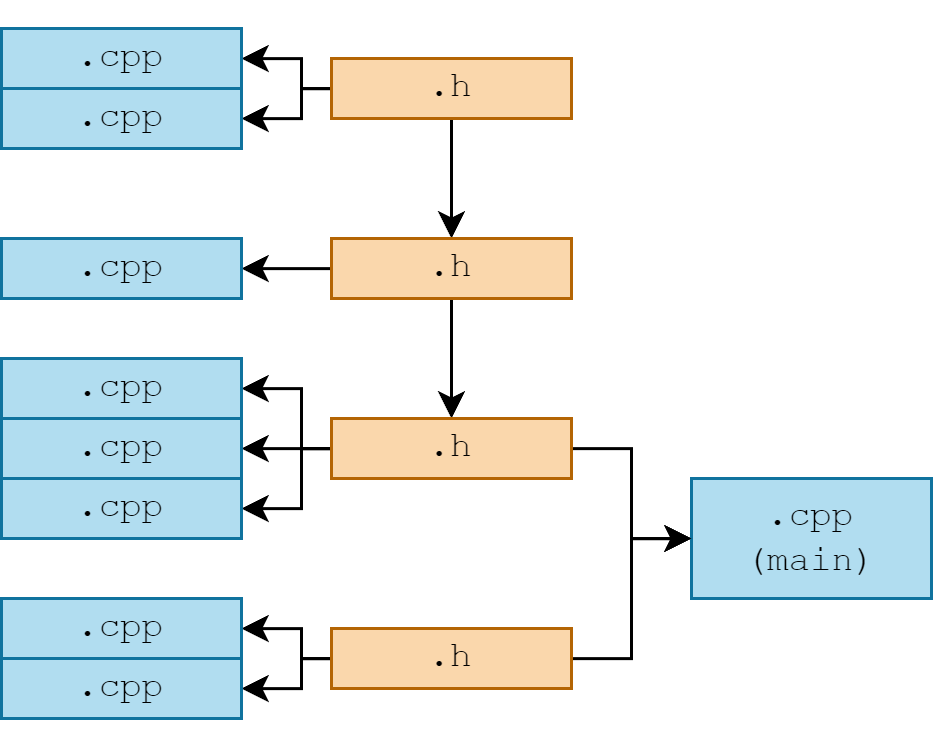
\includegraphics[width=0.6\textwidth]{../images/generalized_parts/07_separate_compilation_300.png}
    \caption{一个跨文件编译的示意图}
    \footnotesize{箭头指向的方向有 \lstinline@#include@ 指令}
\end{figure}
在实际的编程中,我们提倡把下面的内容放在头文件中:
\begin{itemize}
    \item 常量表达式及常量的定义
    \item 结构体和类的定义
    \item 全局函数和成员函数的声明
    \item 函数模板和类模板的定义\footnote{类模板比较特殊,类模板的成员最好定义在头文件中。如果你觉得内容太多,那就把它们组织到不同的头文件中。}
    \item 一些很短的函数(我们可以以内联\footnote{内联(Inline),即用 \lstinline@inline@ 把某个标识符声明为内联。对于函数来说,内联意味着某个具有外部链接的函数在不同翻译单元中都可以有一个定义。编译器会对它们进行优化,我们无需过分纠结。}形式直接定义在头文件中)
\end{itemize}
至于函数的定义,我们可以,而且最好把它们放在其它的源文件中。而 \lstinline@main@ 函数存放在一个单独的源文件中,这样我们就只需要在写好其它函数之后,关注主函数的功能即可。以6.3实操部分的代码为例,我们可以把它拆成这样三个文件:
\lstinputlisting[caption=\texttt{Header.h}]{../code_in_book/7.4-7.6/Header.h}
\lstinputlisting[caption=\texttt{Definition.cpp}]{../code_in_book/7.4-7.6/Definition.cpp}
\lstinputlisting[caption=\texttt{main.cpp}]{../code_in_book/7.4-7.6/main.cpp}
请读者注意各文件之间使用 \lstinline@#include@ 的关系。因为在\texttt{Definition.cpp}中没有使用 \lstinline@using namespace std@,所以我们在定义 \lstinline@transfer@ 函数时,调用 \lstinline@swap@ 函数必须要用 \lstinline@std::swap@ 这样的语法。\par
读者可能会好奇,我们不是在\texttt{Main.cpp}中用过了 \lstinline@using namespace std@ 了吗?不然,因为\texttt{Definition.cpp}和\texttt{Main.cpp}之间没有包含关系,所以\texttt{Main.cpp}中写下的代码不能用在\texttt{Definition.cpp}中,反之亦然。\par
